\documentclass[a4paper]{article}
\usepackage[column]{hedfeatures}
\usepackage[utf8]{inputenc}
\usepackage[russian]{babel}
\usepackage{multirow}
\usepackage{graphicx}

\begin{document}
    \section{Подготовка к работе}
        \begin{enumerate}
            \item На задней панели индикатора установите ось резистора
                <<СМЕЩЕНИЕ>> в крайнее правое положение, что соответствует
                напряжению около 1,1 В. Тумблер <<СМЕЩЕНИЕ>> при этом
                установите в положение <<+>>;
            \item Переключатель ПРЕДЕЛЫ в положение 0;
            \item Кнопка М в нажатом положении;
            \item Кнопка ЛОГ в ненажатом положении;
            \item Кнопка -10dB в ненажатом положении;
            \item Кнопка КОРРЕК в ненажатом положении;
            \item Ручка МЕТКА в среднем положении;
            \item Подайте на разъёмы ПАД. И ОТРАЖ. сигналы соответственно
                падающей и отраженной волн;
            \item Соедините разъём АРМ со входом АРМ ГКЧ.
            \item Включите тумблеры «СЕТЬ» индикатора Я2Р-67 и ГКЧ, и дайте им
                прогреться в течение 20-30 минут.
        \end{enumerate}

        Подготовка и проведение измерений
        \begin{enumerate}
            \item Убедитесь в нормальном функционировании прибора:
                \begin{enumerate}
                    \item должны гореть индикаторы СЕТЬ, ГКЧ и индикатора Я2Р-67;
                    \item должно светиться цифровое табло;
                    \item на экране ЭЛТ индикатора Я2Р-67 должны наблюдаться
                        линия падающей мощности, линия контрольного уровня,
                        линия электронного визира;
                    \item на экране ЭЛТ индикатора Я2Р-67 должны наблюдаться
                        3 числа в соответствии с числами на табло генератора
                        качающей частоты.
                \end{enumerate}
            \item Прибор готов к проведению измерений через 30 минут,
                а калибровку можно начать через 15 минут после включения.
        \end{enumerate}
    \section{Калибровка}

        \begin{enumerate}
            \item При помощи ручек НАЧАЛЬНАЯ ЧАСТОТА и КОНЕЧНАЯ ЧАСТОТА
                установите полный диапазон качания частоты;
            \item Ручкой ОТСЧЁТ индикатора Я2Р-67 установить визир по шкале
                милливольт на отметку 2;
            \item Добейтесь совмещения линии падающей мощности с линией визира,
                с помощью ручек УРОВЕНЬ, МОЩНОСТЬ И ПАД; линия падающей мощности
                должна превратиться в прямую;
            \item Установите переключатель ПРЕДЕЛЫ в положение «0», при этом
                вместо линии падающей мощности на экране ЭЛТ наблюдается линия
                калибровки, регулируемая ручкой КАЛИБР;
            \item Установите ручкой ОТСЧЁТ визир индикатора на отметку 0 дБ
                на шкале dB;
            \item Вращая ручку КАЛИБР, максимально приблизьте линию калибровки
                к линии электронного визира, а при возможности расположите её
                симметрично линии электронного визира;
            \item Измерьте неравномерность линии калибровки, для этого
                совместите ручкой ОТСЧЁТ линию визира с самой верхней \( A_1 \)
                и самой нижней \( A_2 \) точками линии калибровки и проведите
                отсчёт по верхней шкале dB по формуле:
        \end{enumerate}
    \section{Проведение измерений}
    \section{Результаты измерений}
    Определим основные максимумы и минимумы КСВН для пустого волновода,
    волновода с ячменёи и с пшеницей:
    \begin{table}[h]
        \center
        \begin{tabular}{|C{.1}|C{.1}||C{.1}|C{.1}||C{.1}|C{.1}|}
            \hline
            \multicolumn{2}{|c||}{Пустой} &
            \multicolumn{2}{c||}{Пшеница} &
            \multicolumn{2}{|c|}{Ячмень} \\ \hline
            Частота & КСВ & Частота & КСВ & Частота & КСВ \\ \hline
            36.8 & 12 & 36.5 & 2.7  & 36.9 & 2.9  \\ \hline
            37.6 & 6  & 37.4 & 1.48 & 37.7 & 1.9  \\ \hline
            38.2 & 12 & 38.1 & 2.6  & 38.8 & 3.5  \\ \hline
            39.5 & 5  & 39   & 1.5  & 39.6 & 2.6  \\ \hline
            41   & 18 & 39.7 & 2.3  & 40.3 & 3.2  \\ \hline
            41.5 & 16 & 40.6 & 1.54 & 41.2 & 2.1  \\ \hline
            42   & 30 & 41.5 & 2.3  & 41.8 & 2.4  \\ \hline
            42.8 & 14 & 42.4 & 1.62 & 42.8 & 1.36 \\ \hline
            43.7 & 18 & 43.3 & 2.5  & 43.8 & 2    \\ \hline
            45.6 & 6  & 44   & 1.64 & 44.6 & 1.64 \\ \hline
            46.1 & 7  & 44.8 & 2.24 & 46   & 3.2  \\ \hline
            46.4 & 6  & 45.9 & 1.4  & 47.1 & 2.1  \\ \hline
            46.6 & 7  & 46.7 & 1.76 & 47.6 & 2.3  \\ \hline
            47   & 6  & 47.5 & 1.36 & 48.6 & 1.23 \\ \hline
            47.5 & 8  & 48.4 & 1.66 & 49.8 & 2.24 \\ \hline
            48.9 & 14 & 49.6 & 1.31 & 50.5 & 1.72 \\ \hline
                 &    & 50.4 & 1.82 & 51.6 & 2.5  \\ \hline
                 &    & 51.4 & 1.22 &      &      \\ \hline
                 &    & 52.3 & 1.76 &      &      \\ \hline
        \end{tabular}
    \end{table}

    \begin{figure}[h]
        \center
        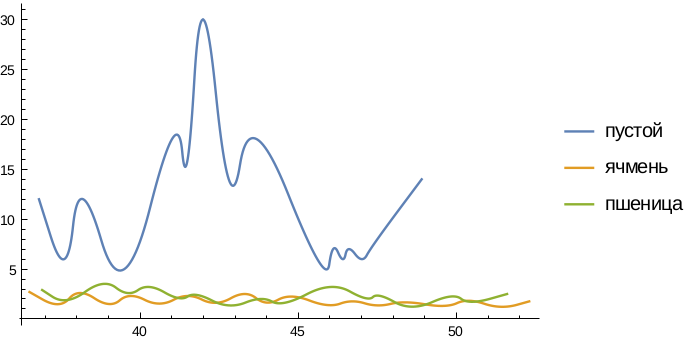
\includegraphics[width=.9\textwidth]{plot1}
        \caption{Зависимость КСВ от частоты}
    \end{figure}

    \begin{figure}[h]
        \center
        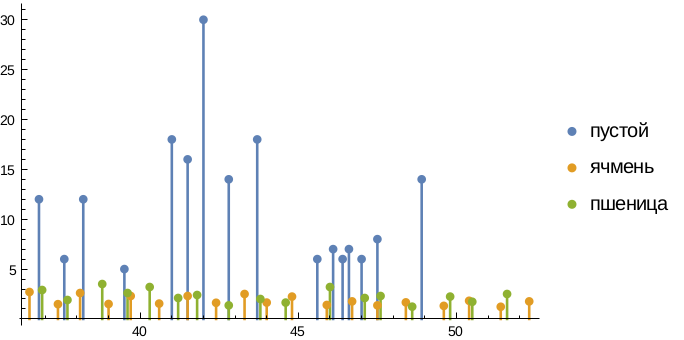
\includegraphics[width=.9\textwidth]{plot2}
        \caption{Зависимость КСВ от частоты}
    \end{figure}

\end{document}
